\begin{center}
	\LARGE{\textbf{Øving 1}}
\end{center}


\section*{Oppgave 1}

\begin{figure}[htb!]
	\centering
	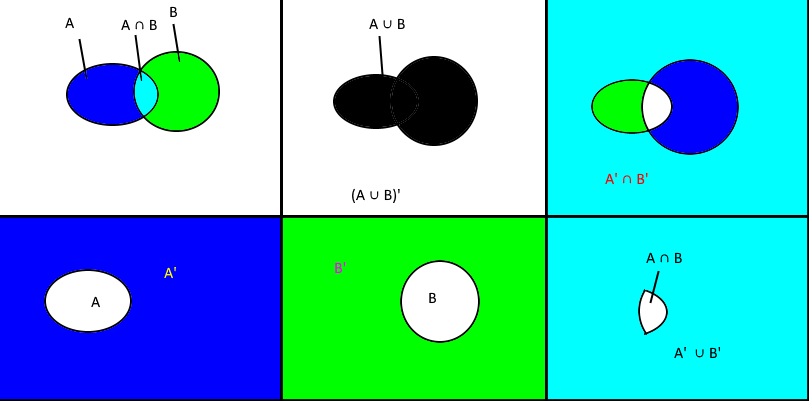
\includegraphics[width = 14cm]{Figurer/1A.png}
	\caption*{de Morgans lov}
	\label{fig:1}
\end{figure}

\begin{figure}[htb!]
	\centering
	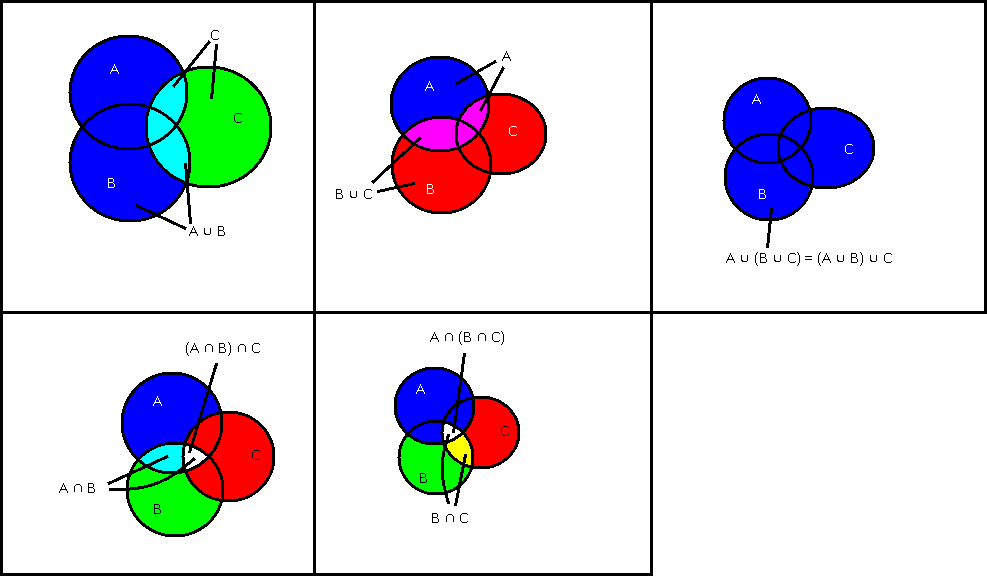
\includegraphics[width = 14cm]{Figurer/1B.png}
\end{figure}

\newpage

\begin{figure}[htb!]
	\centering
	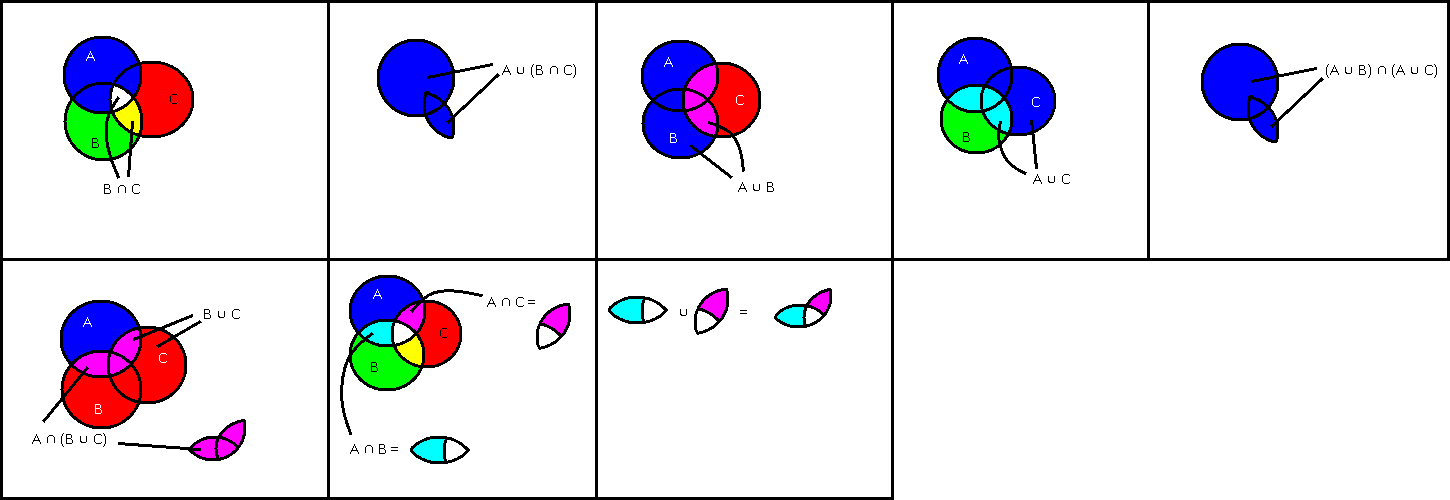
\includegraphics[width = 14cm]{Figurer/1C.png}
\end{figure}


\section*{Oppgave 2}

\begin{gather*}
	\binom{8}{7} = \frac{8!}{1! \cdot 7!} = 8 \\
	\binom{m}{7} = \frac{m!}{7! (m - 7)!} \\
	3 kr \cdot \binom{12}{7} = \frac{12!}{7! \cdot 5!} = 2 376 kr
\end{gather*}


\section*{Oppgave 3}

\begin{gather*}
	B = bildekort \\
	E = ess \\
	Bj = blackjack \\
	P(Bj) = P(B) \cdot P(E) \cdot 2 =
	\frac{16}{52} \cdot \frac{4}{52} \cdot 2 = 4.73\% \\ \\
	P(Bj | E) = \frac{16}{52} = 30.8\% \\ \\
	P(Bj) = 0.06, \quad
	P(E) = 0.1, \quad
	P(E | Bj) = 0.4 \\
	P(Bj | E) = P(E | Bj) \frac{P(Bj)}{P(E)} = 0.4 \cdot \frac{0.06}{0.1} =
	24 \%
\end{gather*}


\newpage


\section*{Oppgave 4}

\subsection*{a)}

\begin{gather*}
	P(E_1) = P(E_2) = 0.01, \quad
	P(E_2 | E_1) = 0.1 \\ \\
	P(E_2 | E_1) \neq P(E_2) => ikke\ uavhengig \\ \\
	P(E_2 | E_1) = \frac{P(E_2 \cap E_1)}{P(E_1)} \neq 0 => ikke\ disjunkte \\ \\
	P(E_2 \cap E_1) = P(E_1) \cdot P(E_2 | E_1) =
	0.01 \cdot 0.1 = 0.001 \\
	P(E_1 \cup E_2) = P(E_1) + P(E_2) - P(E_1 \cap E_2) =
	0.01 + 0.01 - 0.001 = 0.019
\end{gather*}

\subsection*{b)}

\begin{gather*}
	ikke\ tilstrekkelig\ kapasitet = F = \paranth{T \cap \paranth{E_1 \cup E_1}} \cup
	\paranth{\bar{T} \cap E_1 \cap E_2} \\ \\
	P(F) = P(T \cap \paranth{E_1 \cup E_1}) +
	P(\bar{T} \cap E_1 \cap E_2) \\ \\
	P(T \cap \paranth{E_1 \cup E_1}) = P(T) \cdot P(E_1 \cup E_2) =
	0.04 \cdot 0.019 = 0.00076 \\
	P(\bar{T} \cap E_1 \cap E_2) = (1 - P(T)) \cdot P(E_1 \cap E_2) =
	0.96 \cdot 0.001 = 0.00096 \\
	P(F) = 0.00076 + 0.00096 = 0.00172 \\
\end{gather*}


\section*{Oppgave 5}

\begin{gather*}
	P(J) = 0.8, \quad
	P(\bar{J}) = 0.2, \quad
	P(R | J) = 0.02, \quad
	P(R | \bar{J}) = 0.05 \\ \\
	P(J \cap R) = P(J) \cdot P(R | J) = 0.8 \cdot 0.02 = 0.016 \\
	P(\bar{J} \cap R) = P(\bar{J}) \cdot P(R | \bar{J}) = 0.2 \cdot 0.05 = 0.01 \\ \\
	\frac{0.016}{0.01 + 0.016} = 61.5 \%\ av\ innringere\ som\ mener\ ja
\end{gather*}


\newpage


\section*{Oppgave 6}

\begin{gather*}
	P(A \cap B) = P(B) \cdot P(A | B) = 0.09 \cdot 0.5 = 0.045 \\ \\
	P(A \cap \bar B) = P(\bar B) \cdot P(A | \bar B) = 0.91 \cdot 0.01 = 0.0091 \\
	P(A) = P(A \cap B) + P(A \cap \bar B) = 0.045 + 0.0091 = 0.0541 \\ \\
	P(B | A) = P(A | B) \cdot \frac{P(B)}{P(A)} = 0.5 \cdot \frac{0.09}{0.0541} = 0.8312
\end{gather*}

